\documentclass[thesis.tex]{subfiles}

\begin{document}

\iffulldocument\else
	\chapter{KdV5}
\fi

In this chapter, we will look at periodic multi-pulses, which are multi-modal solutions to \cref{eqODE} on a periodic domain. Heuristically, we construct a periodic multi-pulse by gluing together multiple copies of the primary pulse end-to-end in a loop as shown in \cref{fig:permultipulse}.
\begin{figure}
\begin{center}
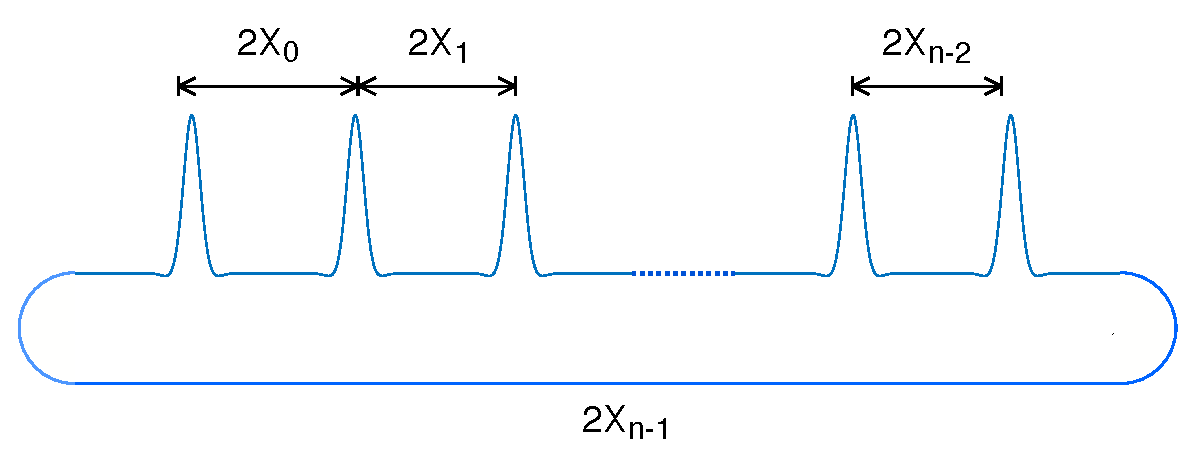
\includegraphics[width=10cm]{periodic/multipulseperiodic}
\end{center}
\caption{Periodic $n-$pulse solution.}
\label{fig:permultipulse}
\end{figure}
We will start by proving the existence of periodic multi-pulses. In the process, we will exhibit a bifurcation structure for periodic 2-pulses. We will then look at their spectral stability, and will apply the result to periodic 2-pulses.

\section{Existence}\label{sec:perexist}

First, we will look at existence. From a spatial dynamics perspective, a periodic multi-pulse is a multi-loop periodic orbit solution $Q_n(x)$ to
\begin{equation}\label{existgenODE}
U'(x) = F(U(x); c)
\end{equation}
which remains close to the primary homoclinic orbit $Q(x)$. A periodic $n$-pulse can be described by $n$ pulse distances $\{X_0, \dots, X_{n-1} \}$, where the distance between consecutive copies of $Q(x)$ in the loop is $2 X_j$. The period of the orbit is $2X$, where $X = X_0 + \dots + X_{n-1}$. A periodic $n$-pulse requires one more pulse distance than an $n$-homoclinic orbit, since we need one more connection to ``close the loop''.  

From a mathematical perspective, rather than describing a periodic multi-pulse by its pulse distances $X_j$, we will adopt an alternative parameterization which is both more convenient and captures the underlying geometry necessary for a periodic $n$-pulse to exist. This parameterization is an adaptation of that in \cite{SandstedeStrut,Sandstede1998} to the periodic case. 

From Hypothesis \ref{hypeqhyp}, the rest state at 0 is a hyperbolic equilibrium point of \cref{existgenODE}. The linearization $DF(0; c)$ about the rest state has a quartet of eigenvalues $\pm \alpha_0 \pm \beta_0 i$, which depends on the wavespeed $c$. All other eigenvalues have real part strictly larger in magnitude than $\alpha_0$. Let
\begin{equation}\label{defrho}
\rho = \frac{\beta_0}{\alpha_0}
\end{equation}
and
\begin{equation}\label{pstar}
p^* = \arctan \rho.
\end{equation}
Define the set
\begin{align}
\mathcal{R} &= \left\{ \exp\left(-\frac{2 k \pi}{\rho}\right) : k \in \N_0 \right\} \cup \{ 0 \},
\end{align}
which is a complete metric space. We will use $r \in \mathcal{R}$ as a scaling parameter. The parameterization is defined as follows.

\begin{definition}\label{def:perparam}
For $n \geq 2$, a \emph{periodic parameterization} of a periodic $n$-pulse is a sequence of parameters $(m_0, \dots, m_{n-1}, \theta)$, where
\begin{enumerate}[(i)]
\item $m_j$ is a nonnegative integer with
\begin{enumerate}
\item at least one of the $m_j \in \{0, 1\}$.
\item $m_{n-1} \geq m_j$ for $j = 0, \dots, n-2$.
\end{enumerate}
\item $\theta \in (\pi + -p^*, p^*]$.
\end{enumerate}
\end{definition}
The selection of $m_{n-1}$ as the largest of the $m_j$ is made only for notational convenience and to allow the parameterization to be unique. Since we are on a periodic domain, there is no loss of generality. The physical pulse distances $X_j$ are determined by these parameters and by the scaling parameter $r$. This works as follows. If $r = \exp\left(-\frac{2 k \pi}{\rho}\right)$, then
\begin{align*}
X_j &= \frac{1}{2 \beta_0}\big( (2 k + m_j)\pi + \theta^*(\theta; m_{n-1} - m_j)\big) + L_0 + \mathcal{O}(r) \\
X_{n-1} &= \frac{1}{2 \beta_0}\big( (2 k + m_{n-1})\pi + \theta \big) + L_0
\end{align*}
where $L_0$ is a constant. The functions $\theta^*(\theta; m): [-\pi + p^*, p^*] \rightarrow \R$ are defined for all nonnegative integers $m$, are continuous in $\theta$, and have the following properties.
\begin{enumerate}[(i)]
\item $\theta^*(0; m) = 0 \text{ for all } m$
\item $|\theta^*(\theta; m)| \leq |\theta|$
\item $|\theta^*(\theta; m)| \leq C \exp\left(-\frac{m \pi}{\rho} \right)$
\item $\theta^*(\theta; 0) = \theta $
\item $\theta^*(p^*; m) = \theta^*(-\pi+p^*; m+1)$ for $m \geq 1$
\end{enumerate}
The last property is a matching condition which ``links up'' the parameterizations corresponding to different $m_j$. These properties, together with the restriction of $\theta$ to the half-open interval $\theta \in (\pi + -p^*, p^*]$, guarantee that each periodic parameterization corresponds to a unique periodic multi-pulse (up to cyclic permutations of the $m_j$; see \cref{remark:cyclicperm} below). The proof that the functions $\theta^*(\theta; m)$ exist and have these properties is given in Lemma \ref{thetaparamlemma} in \cref{perexistproof}. 

We can now state the main theorem of this section, which gives conditions for the existence of periodic multi-pulses. The requirement that the scaling parameter $r$ be sufficiently small means that the individual pulses must be well-separated. The proof is lengthy and is deferred until \cref{perexistproof}.

\begin{theorem}[Existence of $n$-periodic solutions]\label{perexist}
Assume Hypotheses \ref{Ehyp}, \ref{Hhyp}, \ref{hypeqhyp}, \ref{Qexistshyp}, and \ref{H0transversehyp}. Let $Q(x)$ be the transversely constructed, symmetric primary pulse solution to \eqref{genODE} from Hypothesis \ref{Qexistshyp}. For any periodic parameterization $(m_0, \dots, m_{n-1}, \theta)$ with $\theta \notin \{-\pi + p^*, p^* \}$, there exists $r_* = r^*(m_0, \dots, m_{n-1}, \theta) > 0$ such that for any $r \in \mathcal{R}$ with $r \leq r_*$:
\begin{enumerate}[(i)]
	\item There exists a periodic $n$-pulse solution $Q_n(x) = Q_n(x; m_0, \dots, m_{n-1}, \theta, r)$ to \eqref{genODE}.

	\item The distances between consecutive copies of $Q(x)$ are $2X_j$, where
	\begin{align}\label{Xj}
		X_j(r; m_j, m_{n-1},\theta) &= \frac{1}{2 \alpha_0} |\log r| + \frac{1}{2\beta_0} t_j(r; m_j,m_{n-1}, \theta) + L_0 && j = 0, \dots, n-2 \\
		X_{n-1}(r; m_{n-1}, \theta) &= \frac{1}{2 \alpha_0} |\log r| + \frac{1}{2 \beta_0}\big( m_{n-1}\pi + \theta \big) + L_0.
	\end{align}
	The $t_j(r; m_j, m_{n-1}, \theta): \mathcal{R} \rightarrow \R$ are continuous in $r$ with 
	\[
	t_j(0; m_j, \theta) = m_j \pi + \theta^*(\theta; m_{n-1} - m_j),
	\]
	and $L_0$ is a constant.

	\item The periodic domain has length $2X$, where
	\begin{align}\label{Xdomain}
	X(r; m_0, \dots, m_{n-1}, \theta) = \frac{n}{2\alpha_0} |\log r| + \frac{1}{2\beta_0} \sum_{j=0}^{n-1} t_j(r; m_j, \theta) + n L_0
	\end{align}

	\item $Q_n(x)$ can be written as piecewise perturbation of the primary pulse $Q(x)$. Details are given below in Lemma \ref{solvewithjumps}.
\end{enumerate}
\end{theorem}

\begin{remark}\label{remark:cyclicperm}
The periodic $n$-pulses constructed in \cref{perexist} are unique up to ``rotation'' of the integers $(m_0, \dots, m_{n-1})$ in the periodic parameterization. For example, $(m_0, m_1, m_2, \theta)$, $(m_2, m_0, m_1, \theta)$, and $(m_1, m_2, m_0, \theta)$ all give the same solution.
\end{remark}

The condition that $\theta \notin \{-\pi + p^*, p^*) \}$ in \cref{perexist} is used to avoid any bifurcation points which may arise in the construction. For periodic 2-pulses, we can use a symmetry argument to give a complete bifurcation picture. In the next theorem, we state an existence result for periodic 2-pulses and show that asymmetric solutions bifurcate from symmetric solutions in a series of pitchfork bifurcations. This is illustrated in the left panel of \cref{fig:2pitch}. 
\begin{figure}
\begin{center}
\begin{tabular}{cc}
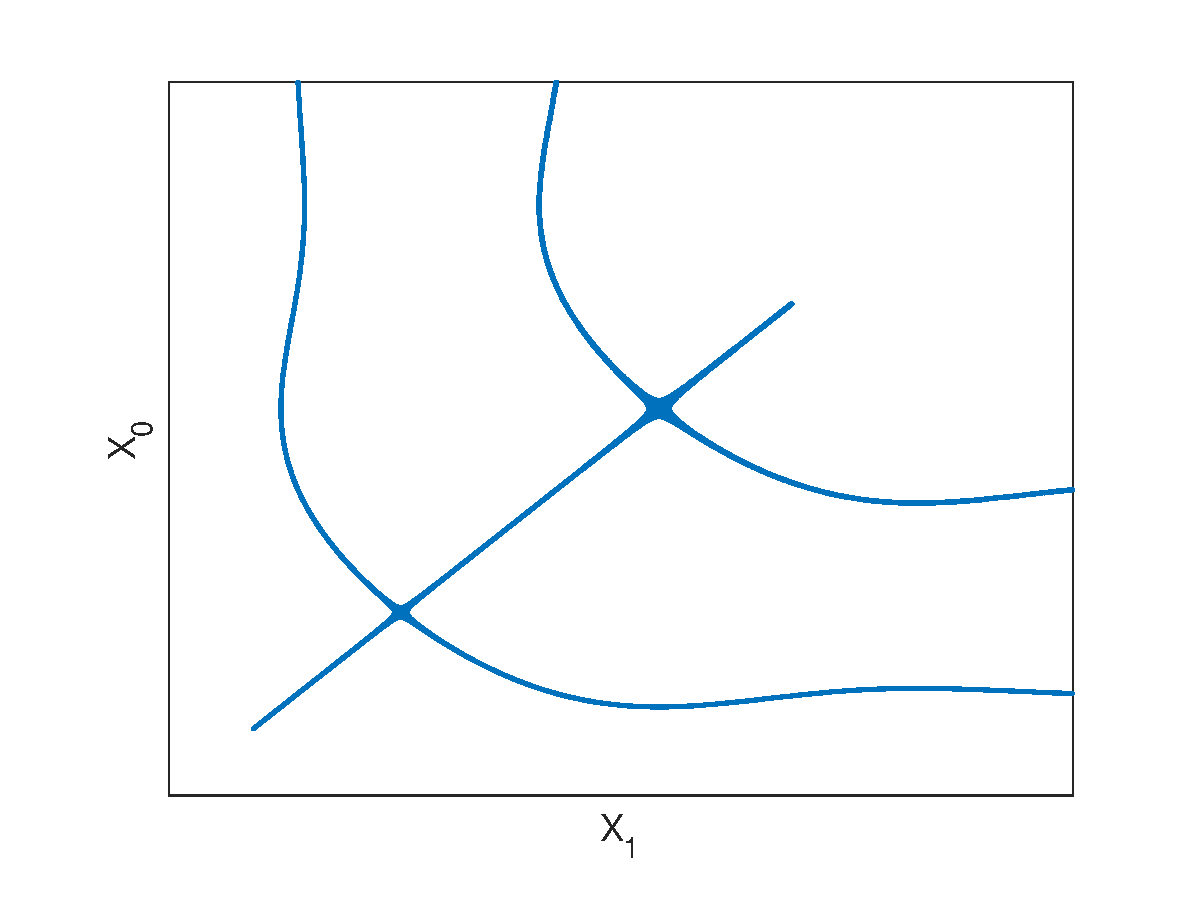
\includegraphics[width=8cm]{periodic/2pitchfork.eps}
\includegraphics[width=8cm]{periodic/2pitchparam1}
\end{tabular}
\end{center}
\caption[Pitchfork bifurcation structure for periodic 2-pulses]{Pitchfork bifurcation structure for periodic 2-pulses (right panel). Parameterization from \cref{2pulsebifurcation} (left panel). Symmetric periodic 2-pulses are in blue, and asymmetric periodic 2-pulses are in orange. Parameters $s_0$ and $s_1$ increase in the direction of the arrow.}
\label{fig:2pitch}
\end{figure} 
We use a different parameterization than in \cref{perexist}, which is illustrated in the right panel of \cref{fig:2pitch}. The proof this theorem is at the end of \cref{perexistproof}.

\begin{theorem}\label{2pulsebifurcation}
Assume Hypotheses \ref{Ehyp}, \ref{Hhyp}, \ref{hypeqhyp}, \ref{Qexistshyp}, and \ref{H0transversehyp}. Let $Q(x)$ be a transversely constructed, symmetric primary pulse solution to \eqref{genODE}. There exists $r_* > 0$ such that for all $r \in \mathcal{R}$ with $r \leq r_*$ and $m_0 \in \{0, 1\}$
\begin{enumerate}[(i)]
	\item There exists a family of symmetric periodic 2-pulses $\tilde{Q}_2(x; m_0, s_0, r)$ parameterized by $s_0 \in [0, \pi)$. The distances $\tilde{X}_j$ are given by
	\begin{equation}\label{2psymmdist}
		\tilde{X}_0(r, s_0) = \tilde{X}_1(r, s_0) = \frac{1}{2 \alpha_0} |\log r| + \frac{\pi}{2\beta_0} (m_0 + s_0) + L_0.
	\end{equation}
	\item There exists a family of asymmetric periodic 2-pulses $Q_2(x; m_0, s_1, r)$ with distances $X_1 > X_0$ parameterized by $s_1 \in [p^*, \infty)$. The distances $X_j$ are given by
	\begin{equation}\label{2pasymmdist}
	\begin{aligned}
		X_0(r, m_0, s_1) &= \frac{1}{2 \alpha_0} |\log r| + \frac{1}{2\beta_0} t_0(r; m_0, s_1) + L_0 \\
		X_1(r, s_1) &= \frac{1}{2 \alpha_0} |\log r| + \frac{1}{2\beta_0} s_1 + L_0, 
	\end{aligned}
	\end{equation}
	where $t_0(r; m_0, s_1)$ is continuous in $r$ and $t_1$, and $t_0(0; m_0, k \pi) = m_0$ for all nonnegative integers $k$. Furthermore,
	\begin{align}\label{deft0}
	t_0(0; m_0, s_1) = m_0 \pi + \mathcal{O}\left(-\frac{1}{\rho} s_1 \right)
	\end{align}
	The periodic domain has length $2X$, where
	\begin{equation}\label{X2pdomain}
	X(r, m_0, s_1) = \frac{1}{2 \alpha_0} 2 |\log r| + \frac{1}{2\beta_0} \left( t_0(r; m_0, s_1) + s_1\right) + 2 L_0.
	\end{equation}

	\item The two families meet at a pitchfork bifurcation. In terms of the two parameterizations, this occurs when $s_0 = p^*(m_0; r)$ and $s_1 = p^*$. The bifurcation points $p^*(m_0; r)$ are continuous in $r$, and
	\[
	p^*(m_0; r) \rightarrow \arctan \rho \text{ as }r \rightarrow 0.
	\]
\end{enumerate}
\end{theorem}

\section{Spectral stability}\label{sec:perstab}

In this section, we look at the spectral stability of the periodic multi-pulses which we constructed in the previous section. To do this, we will adapt the framework we set up in \cref{sec:genspectrum}.

Let $Q(x)$ be the primary pulse solution. Let $Q_n(x)$ be any periodic multi-pulse solution constructed according to Theorem \ref{perexist}, and let $X$ be given by \cref{Xdomain}. Let $q_n(x)$ be the first component of $Q_n(x)$. We are interested in the PDE eigenvalue problem
\begin{equation}\label{genPDEeigper}
\partial_x \calL(q_n) v = \lambda v
\end{equation}
resulting from the linearization of the original PDE \cref{genPDE} about $q_n(x)$. It is natural to pose \cref{genPDEeigper} on the space of periodic functions $H^{2m}_{\text{per}}[-X,X]$, where
\[
H^{2m}_{\text{per}}[-X,X] = \left\{ f \in H^{2m}(\R) : f^{(k)}(-X) = f^{(k)}(X) \text{ for } k = 0, \dots, 2m \right\} 
\]
The norm on this space is the $H^{2m}$ norm restricted to $[-X, X]$. 

As in \cref{sec:genspectrum}, we use a spatial dynamics formulation and write the PDE eigenvalue problem \cref{genPDEeigper} as the first order system of ODEs
\begin{equation}\label{PDEeigsystemper2}
\begin{aligned}
V'(x) &= A(Q_n(x))V(x) + \lambda B V(x) \\
V(-X) &= V(X)
\end{aligned}
\end{equation}
where $V(x) \in C^0(\R,\R^{2m+1})$, and we have imposed an additional periodic constraint on $V(x)$. To aid in the analysis, we rewrite \cref{PDEeigsystemper2} as
\begin{equation}\label{PDEeigsystemper3}
\begin{aligned}
V'(x) &= A(Q_n(x); \lambda)V(x) \\
V(-X) &= V(X),
\end{aligned}
\end{equation}
where 
\begin{equation}\label{AQnlambda}
A(Q_n(x); \lambda) = A(Q_n(x)) + \lambda B.
\end{equation}
Let $A(\lambda) = A(0; \lambda)$. By Lemma \ref{eigA0lemma}, $A(0)$ has a simple eigenvalue at 0. The next lemma states that for small $\lambda$, $A(\lambda)$ has a simple eigenvalue $\nu(\lambda)$ near 0; it is proved as part of Lemma \ref{nulambdalemma} in \cref{blockmatrixproof}.

% nu(lambda) lemma
\begin{lemma}\label{nulambdalemmasimple}
There exists $\delta_0 > 0$ such that for $|\lambda| < \delta_0$, the matrix $A(\lambda)$ has a simple eigenvalue $\nu(\lambda)$ near 0.
\end{lemma}

We can now state the main theorem of this section, which provides a condition for \cref{PDEeigsystemper3} to have a solution. Since the spatial dynamics formulation \cref{PDEeigsystemper3} is equivalent to the PDE eigenvalue problem, this allow us to find the eigenvalues of \cref{genPDEeigper}. This theorem is analogous to \cite[Theorem 2]{Sandstede1998}, where the matrix $S(\lambda)$ is replaced by a block matrix. The proof is lengthly and is deferred until \cref{blockmatrixproof}.

% block matrix theorem
\begin{theorem}\label{blockmatrixtheorem}
Assume Hypotheses \ref{Ehyp}, \ref{Hhyp}, \ref{hypeqhyp}, \ref{Qexistshyp}, and \ref{H0transversehyp}, \ref{Qclocalhyp}, and \ref{Melnikov2hyp}. Let $Q(x)$ be the primary pulse solution, and let $\Psi(x)$ be the solution to the adjoint variational equation from Lemma \ref{varadjsolutions}. Choose any periodic parameterization $(m_0, \dots, m_{n-1}, \theta)$ with $\theta \neq \pm \pi$, and let $r_*$ be as in \cref{perexist}. 

Choose any positive integer $N$. Then for any $r \leq r_*$ there exists $\delta(r,N)$, where $0 < \delta(r,N) < N/|\log r|$, with the following property. There exists a bounded, nonzero solution $V(x)$ of \cref{PDEeigsystemper3} for $|\lambda| < \delta(r,N)$ if and only if
\begin{equation}\label{blockmatrixcond}
E(\lambda) = \det S(\lambda) = 0.
\end{equation}
$S(\lambda)$ is the $(2n \times 2n)$ block matrix
\begin{equation}\label{blockeq}
S(\lambda) = 
\begin{pmatrix}
K(\lambda) + C_1 & \lambda K_2(\lambda) - \lambda^2 \tilde{M}^c I + D_1 \\
-\frac{1}{2} \lambda M^c K_1(\lambda) + C_2 & A - \lambda^2 MI + D_2
\end{pmatrix}
\end{equation}
The individual terms in $S(\lambda)$ are as follows.

\begin{enumerate}
\item $K(\lambda)$ is the periodic, bi-diagonal matrix
\begin{align*}
K(\lambda) =  
\begin{pmatrix}
e^{-\nu(\lambda)X_1} & & & & & -e^{\nu(\lambda)X_0} \\
-e^{\nu(\lambda)X_1} & e^{-\nu(\lambda)X_2} \\
& -e^{\nu(\lambda)X_2} & e^{-\nu(\lambda)X_3} \\
  & & \ddots & && \\
& & & & -e^{\nu(\lambda)X_{n-1}} & e^{-\nu(\lambda)X_0}
\end{pmatrix}
\end{align*}
where $\nu(\lambda)$ is defined in Lemma \ref{nulambdalemmasimple}.

\item $K_1(\lambda)$ is the same matrix as $K(\lambda)$ with all terms positive.

\item $A$ is the symmetric banded matrix
\begin{align}\label{Asymm}
A &= \begin{pmatrix}
-a_{n-1} - a_0 & a_0 & & &  & a_{n-1}\\
a_0 & -a_0 - a_1 &  a_1 \\
& a_1 & -a_1 - a_2 &  a_2 \\
& \ddots & \ddots & \ddots \\
a_{n-1} & & & & a_{n-2} & -a_{n-2} - a_{n-1} \\
\end{pmatrix}
\end{align}
where
\begin{align*}
a_i &= \langle \Psi(X_i), Q'(-X_i) \rangle
\end{align*}

\item $K_2(\lambda)$ is the matrix
\begin{align*}
K_2(\lambda) &= \begin{pmatrix}
k_0^+ - k_1^- & k_1^- &&& -k_0^+ \\
-k_1^+ & k_1^+ - k_2^- & k_2^- \\
& -k_2^+ & k_2^+ - k_3^- & k_3^- \\ && \ddots \\
\\
k_0^- &&& -k_{n-1}^+ & k_{n-1}^+ - k_0^- 
\end{pmatrix}
\end{align*}
with entries
\begin{align*}
k_i^- &= e^{-\nu(\lambda)X_i} q(X_i)\\
k_i^+ &= e^{\nu(\lambda)X_i} q(X_i),
\end{align*}
where $q(x)$ is the first component of the primary pulse solution $Q(x)$. 

\item $M$, $M^c$, $\tilde{M}$, and $\tilde{M}^c$ are  Melnikov-type integrals
\begin{align*}
M &= \int_{-\infty}^\infty q(y) \partial_c q(y) dy \\
M^c &= \int_{-\infty}^\infty q(y) v^c(y) dy \\
\tilde{M}^c &= \int_{-\infty}^\infty \partial_c q(y) dy
\end{align*}
where $v^c(y)$ is the first component of $V^c(y)$, which is defined in \cref{varadjsolutions}.

\item The remainder matrices and $K_2(\lambda)$ are analytic in $\lambda$ and have uniform bounds
\begin{align*}
|K_2(\lambda)| &\leq C r^{1/2} \\
|C_1| &\leq C |\lambda|(|\lambda| + r^{1/2}) \\
|D_1| &\leq C |\lambda|(|\lambda| + r^{1/2})^2 \\
|C_2| &\leq C (|\lambda| + r^{1/2})^2 \\
|D_2| &\leq C (|\lambda| + r^{1/2})^3 
\end{align*}
The constants $C$ depend on $N$.
\end{enumerate}
\end{theorem}

\begin{remark}
In \cref{blockmatrixtheorem}, we restricted $|\lambda|$ to $|\lambda| < N/|\log r|$, for a positive integer $N$ we choose. Without this restriction, the analysis is still possible, but the remainder terms in \cref{blockeq} are much more complicated.
\end{remark}

To leading order, equation \cref{blockeq} is block diagonal with blocks $A - \lambda^2 MI$ and $K(\lambda)$. As in \cref{chapter:kdv5homoclinic}, we expect that points where $A - \lambda^2 MI$ is singular will give us interaction eigenvalues as well as two kernel eigenvalues. In addition, we expect to find another set of eigenvalues at the points where $K(\lambda)$ is singular, which are
\begin{align*}
\lambda &= c\frac{k \pi i}{X} && k \in \Z.
\end{align*}
This will be a set of discrete, purely imaginary eigenvalues (which will include one more kernel eigenvalue). Since these are the periodic analogue of the essential spectrum in the $n$-homoclinic case, we will refer to these as essential spectrum eigenvalues, even though they are technically still part of the point spectrum. 

\begin{remark}
For any positive integer $N$ we choose, it follows from \cref{Xdomain} that for all $r \leq r_*$,
\begin{align*}
\left| c\frac{k \pi i}{X} \right| \leq \delta(r,N) && k \in \Z, |k|\leq N.
\end{align*}
Thus the restriction $\delta(r,N) < N/|\log r|$ in \cref{blockmatrixtheorem} will not hinder a search for the first $N$ essential spectrum eigenvalues.
\end{remark}

\section{Spectrum of periodic 2-pulse}\label{sec:per2peig}

We will apply \cref{blockmatrixtheorem} to the simplest case, which is the periodic 2-pulse. All proofs from this section are in \cref{per2pproof}. The block matrix $S(\lambda)$ is a $4\times 4$ matrix, the form of which is given in the next corollary, which follows immediately from \cref{blockmatrixtheorem}.

\begin{corollary}\label{corr:2blockmatrix}
For a periodic 2-pulse, the block matrix \cref{blockeq} from \cref{blockmatrixtheorem} can be written as $S(\lambda) = S_1(\lambda) + S_2(\lambda)$. $S_1(\lambda)$ is the $4 \times 4$ matrix
\begin{align}
S&_1(\lambda) = \\
&\begin{pmatrix}
e^{-\nu(\lambda)X_1} & -e^{\nu(\lambda)X_0} & k_0^+ - k_1^- -\tilde{M}^c \lambda^2 & -k_0^+ + k_1^- \\
-e^{\nu(\lambda)X_1} & e^{-\nu(\lambda)X_0} & k_0^- - k_1^+ & -k_0^- + k_1^+-\tilde{M}^c \lambda^2 \\
-\frac{1}{2}\lambda M^c e^{-\nu(\lambda)X_1} & -\frac{1}{2}\lambda M^ce^{\nu(\lambda)X_0} &-a-\lambda^2 M_2 & a \\
-\frac{1}{2}\lambda M^c e^{\nu(\lambda)X_1} & -\frac{1}{2}\lambda M^c e^{-\nu(\lambda)X_0}  & a & -a-\lambda^2 M_2 \\
\end{pmatrix}
\end{align}
where
\begin{equation}\label{2pa}
a = \langle \Psi(X_0), Q'(-X_0) \rangle + \langle \Psi(X_1), Q'(-X_1) \rangle
\end{equation}
and the rest of the terms are defined in \cref{blockmatrixtheorem}. $S_2(\lambda)$ is the remainder matrix
\[
S_2(\lambda) = \begin{pmatrix} C_1 & D_1 \\ C_2 & D_2 \end{pmatrix}.
\]
The remainder terms have the same bounds as in \cref{blockmatrixtheorem}.
\end{corollary}

With the aid of Mathematica, the determinant of the block matrix for the periodic 2-pulse is a straightforward computation.

\begin{corollary}\label{corr:2perDet1}
For a periodic 2-pulse, the determinant of the block matrix $S(\lambda)$ is given by
\begin{equation*}
\begin{aligned}
\det S(&\lambda) = -2 \lambda^2 M (2a + \lambda^2 M) \sinh(\nu(\lambda)X) + R(\lambda),
\end{aligned}
\end{equation*}
where the remainder term have bounds
\begin{align*}
|R(\lambda)| \leq C(r^{1/2} + |\lambda|)^5
\end{align*}
\end{corollary}

The interaction eigenvalue pattern will be determined by the quantity $a$ in \cref{2pa}. In order to characterize this, we will need to make one technical hypothesis. Define the functions $H: \R^+ \times \R^+ \rightarrow \R$ and $K: \R^+ \times \R^+ \rightarrow \R$ by 
\begin{align}
H(b_0, b_1) &= b_0 \sin \left( -\rho \log b_0 \right) - b_1 \sin \left( -\rho \log b_1 \right) \label{perdefH} \\
H_1(b_0, b_1) &= b_0 \left[ \rho \cos \left( -\rho \log b_0 \right) - \sin \left( -\rho \log b_0 \right) \right] + b_1 \left[ \rho \cos \left( -\rho \log b_1 \right) - \sin \left( -\rho \log b_1 \right) \right]  \label{perdefH1} \\
\end{align}
Roughly speaking, the permissible pulse distances for periodic 2-pulses are determined by the zero set of $H(b_0, b_1)$. See \cref{section:bifH} for details. The value of $a$ is determined by $H_1(b_0, b_1)$ evaluated on the zero set of $H(b_0, b_1)$. We hypothesize that the zero sets of these two functions overlap only at a discrete set of points corresponding the the pitchfork bifurcation points in \cref{2pulsebifurcation}.

\begin{hypothesis}\label{Hoverlaphyp}
The zero sets of $H(b_0, b_1)$ and $H_1(b_0, b_1)$ intersect only at the discrete set of points
\begin{align*}
(b_0, b_1) &= (b_k^*, b_k^*) && k \in \Z
\end{align*}
where 
\begin{equation*}
b^*_k = e^{-\frac{1}{\rho} (k \pi + p^*) }
\end{equation*}
These are the same as the pitchfork bifurcation points from \cref{2pulsebifurcation}.
\end{hypothesis}

\begin{remark}There is strong numerical evidence that \cref{Hoverlaphyp} is true. See \cref{fig:HH1overlap} for a plot of two zero sets. Although it is likely that \cref{Hoverlaphyp} can be proved, the functions involved, while smooth, are not well-behaved, making the analysis very difficult.
\end{remark}

\begin{figure}
\begin{center}
\begin{tabular}{cc}
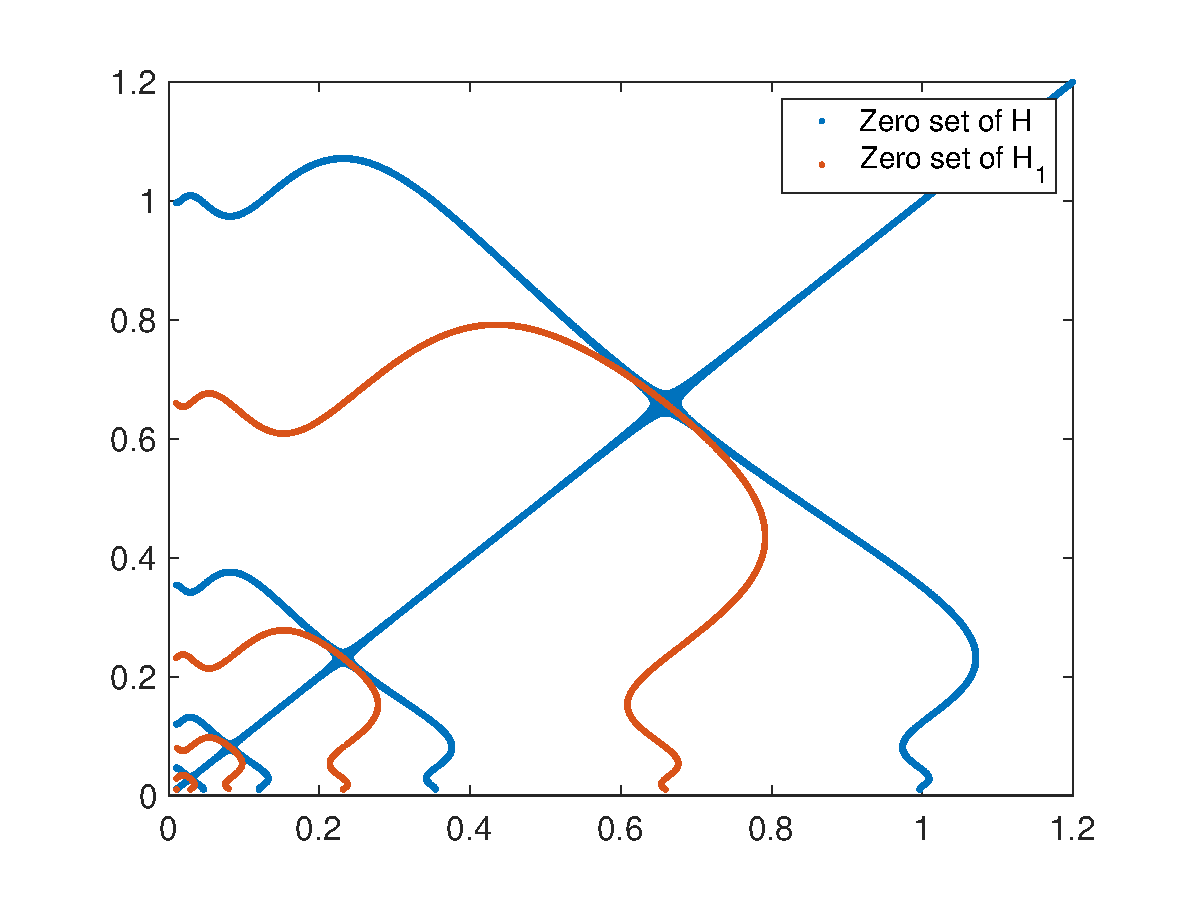
\includegraphics[width=10cm]{images/periodic/zeroHoverlap.eps} 
\end{tabular}
\end{center}
\caption{ Zero sets of $H(b_0, b_1)$ (blue) and $H_1(b_0, b_1)$ (orange). }
\label{fig:HH1overlap}
\end{figure}

We can now characterize the quantity $a$ in \cref{2pa} from \cref{corr:2blockmatrix}.

\begin{lemma}\label{lemma:chara}
Let $r_*$ be as in Theorem \ref{2pulsebifurcation}. Then for any $r \in \mathcal{R}$ with $r \leq r_*$:
\begin{enumerate}[(i)]
	\item For a symmetric periodic 2-pulse $\tilde{Q}_2(x; m_0, s_0, r)$, $a = r \tilde{a}(r; m_0, s_0)$, where $\tilde{a}(r; m_0, s_0)$ is continuous in $r$. Furthermore $\tilde{a}(0; m_0, s_0) = 0$ if and only if $s_0 = p^*$. For $s_0 \neq p^*$,
	\begin{equation}
	\begin{aligned}
	\text{if }s_0 &> p^*, \, \tilde{a}(0; 0, s_0) > 0 \text{ and } \tilde{a}(0; 1, s_0) < 0 \\
	\text{if }s_0 &< p^*, \, \tilde{a}(0; 0, s_0) < 0 \text{ and } \tilde{a}(0; 1, s_0) > 0 
	\end{aligned}
	\end{equation}

	\item For an asymmetric periodic 2-pulse $Q_2(x; m_0, s_1, r)$, $a = r \tilde{a}(r; m_0, s_1)$, where $\tilde{a}(r; m_0, s_0)$ is continuous in $r$. The sign of $\tilde{a}(r; m_0, s_0)$ is completely determined by $m_0$ as follows.
	\begin{equation} 
	\begin{aligned}
	\tilde{a}(0; m_0, s_1) &< 0 && \text{if }m_0 = 0 \\
	\tilde{a}(0; m_0, s_1) &> 0 && \text{if }m_0 = 1
	\end{aligned}
	\end{equation}
	Furthermore,
	\begin{equation}\label{tildeas1limit}
	\tilde{a}(r; m_0, s_1) = \tilde{a}^*(m_0) + \mathcal{O}\left(r^{\gamma/2\alpha_0} + e^{-\frac{1}{\rho}s_1} \right),
	\end{equation}
	where $\gamma > 0$. Finally, $\tilde{a}^*(m_0) < 0$ if $m_0 = 0$ and $\tilde{a}^*(m_0) > 0$ if $m_0 = 1$.
\end{enumerate}	
\end{lemma}

We will consider only the case where the interaction eigenvalues are ``out of the way'' of the essential spectrum eigenvalues. Since the interaction eigenvalues scale like $r^{1/2}$ and the essential spectrum eigenvalues scale like $1/|\log r|$, we can always choose $r$ sufficiently small so that this is the case. In particular, this will always avoid the Krein bubbles that we observed numerically in \cref{chapter:KdV5numerics}. We will discuss the Krein bubbles in the concluding chapter. We expect that the eigenvalues will come in one of the two patterns shown in \cref{fig:2ppatterns}.

\begin{figure}
\begin{center}
\begin{tabular}{cc}
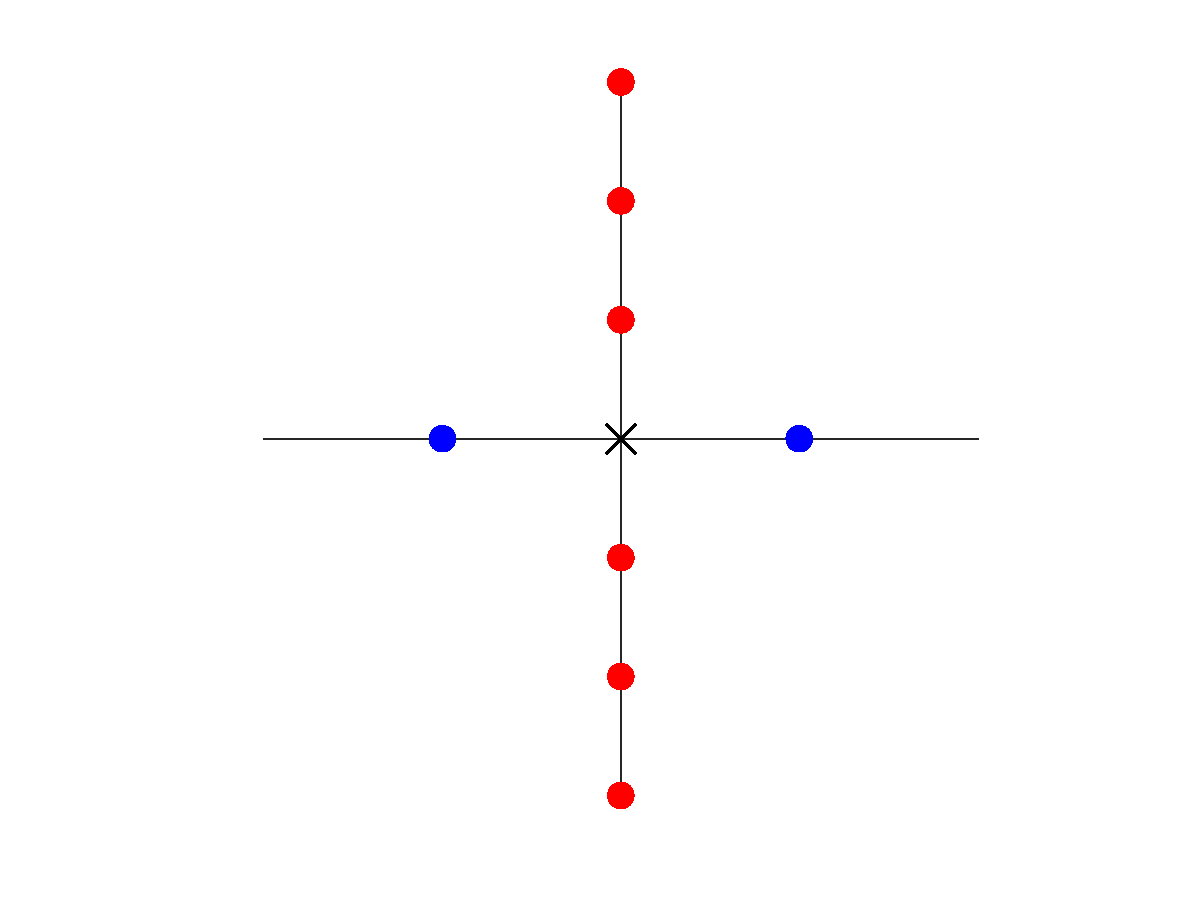
\includegraphics[width=5cm]{images/kdv5/2punstableeigpattern.eps} &
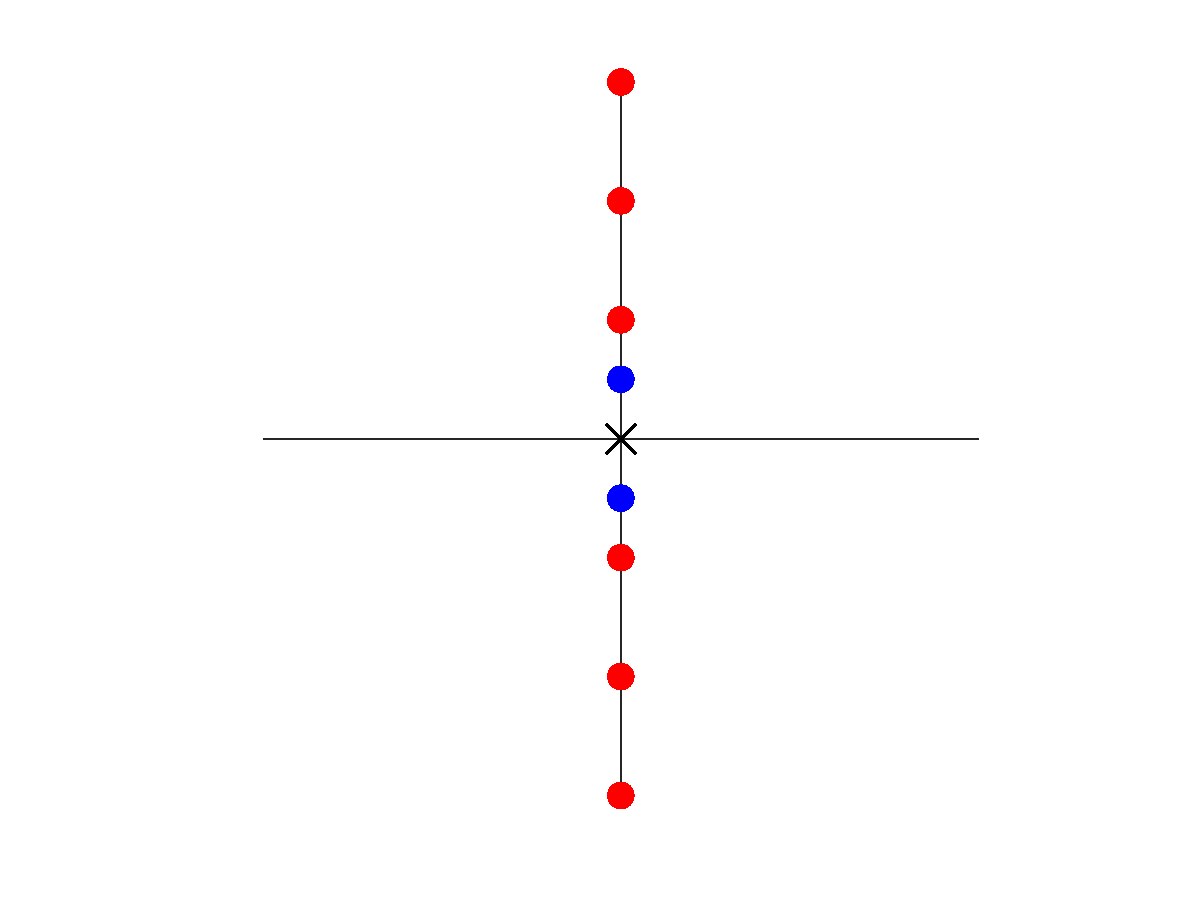
\includegraphics[width=5cm]{images/kdv5/2pstableeigpattern.eps} 
\end{tabular}
\caption{Eigenvalue patterns for periodic 2-pulse with essential spectrum out of the way. Blue dots are interaction eigenvalues, red dots are essential spectrum eigenvalues, and black X at the origin represents the three kernel eigenvalues. Left panel shows a pair of real interaction eigenvalues, and right panel shows a pair of purely imaginary interaction eigenvalues.}
\label{fig:2ppatterns}
\end{center}
\end{figure}

We will state the result separately for asymmetric and symmetric periodic 2-pulses. First, we locate the eigenvalues for asymmetric 2-pulses. As long as $r$ is chosen sufficiently small, the interaction eigenvalue pattern is determined by the parameter $m_0$, and the essential spectrum eigenvalues do not interfere.

\begin{theorem}\label{theorem:2peigsassym}
Assume Hypotheses \ref{Ehyp}, \ref{Hhyp}, \ref{hypeqhyp}, \ref{Qexistshyp}, \ref{H0transversehyp}, \ref{Qclocalhyp}, \ref{Melnikov2hyp}, and \ref{Hoverlaphyp}. Let $r_*$ be as in \cref{2pulsebifurcation}. Let $\tilde{a}(r)$ be as in \cref{lemma:chara}. Choose any integer $N > 0$, and let $\delta(N,r)$ be as in Theorem \ref{blockmatrixtheorem}. Then for every $m_0 \in \{0, 1\}$ and $s_1 > p^*$ there exists $r_1 = r_1(m_0, s_1, N) \leq r_*$ with the following property. For any $r \in \mathcal{R}$ with $r \leq r_1$, the following hold regarding the spectrum associated with the asymmetric periodic 2-pulse $Q_2(x; m_0, s_1, r)$.

\begin{enumerate}[(i)]
\item There is an eigenvalue at 0 with algebraic multiplicity 3. 
\item Let $N_1 \leq N$ be the largest positive integer such that $N_1/|\log r| < \delta(N,r)$. Then there are $2N_1$ nonzero essential spectrum eigenvalues $\lambda = \{ \pm \lambda_m^{\text{ess}} : m = 1, \dots, N_1 \}$, where
\[
\lambda_m^{\text{ess}}(r) = c \frac{m \pi i}{X}+  \mathcal{O}\left( \frac{1}{|\log r|^2} \right)
\]
is on the imaginary axis and $X$ is given by \cref{Xdomain}.

\item There is a pair of interaction eigenvalues located at $\lambda = \pm \lambda^{\text{int}}(r)$, where
	\begin{align*}
	\lambda^{\text{int}}(r) =  \sqrt{-\frac{2 \tilde{a}(r)}{M}}r^{1/2} + \mathcal{O}\left( \frac{r^{1/2}}{|\log r|} \right) 
	\end{align*}
and $|\lambda^{\text{int}}(r)| < \frac{1}{2}|\lambda_1^{\text{ess}}(r)|$. If $M > 0$, these are real when $m_0 = 0$ and purely imaginary when $m_0 = 1$. (This is reversed if $M < 0)$. 
\item There are no other eigenvalues inside a circle with radius slightly larger than $|\lambda_{N_1}^{\text{ess}}(r)|$.
\end{enumerate}
\end{theorem}

Next, we consider the symmetric periodic 2-pulse. As long as we are away from the pitchfork bifurcation points, i.e. as long as $\tilde{a}(0) \neq 0$, the results of \cref{theorem:2peigsassym} hold in the symmetric case as well; the only difference is that the eigenvalue pattern is determined by the sign of $\tilde{a}_0(0)$ rather than by $m_0$. Thus we only need to consider what happens at the pitchfork bifurcation point.

\begin{theorem}\label{theorem:2peigssym}
Assume Hypotheses \ref{Ehyp}, \ref{Hhyp}, \ref{hypeqhyp}, \ref{Qexistshyp}, \ref{H0transversehyp}, \ref{Qclocalhyp}, \ref{Melnikov2hyp}, and \ref{Hoverlaphyp}. Let $r_*$ be as in \cref{2pulsebifurcation}. Then there exists $r_1 \leq r_*$ such that for all $r \in \mathcal{R}$ with $r \leq r_1$ and for $m_0 \in \{0, 1\}$, there is eigenvalue at 0 with algebraic multiplicity 5 for the symmetric periodic 2-pulse $\tilde{Q}_2(x; m_0, p^*(r), r)$.
\end{theorem}

\iffulldocument\else
	\bibliographystyle{amsalpha}
	\bibliography{thesis.bib}
\fi

\section{Spectrum of periodic multi-pulses}

When $n \geq 3$, it should be possible to prove an analogue to \cref{theorem:2peigsassym} in the case where the essential spectrum eigenvalues and nonzero interaction eigenvalues do not interfere with each other. Since it is too unwieldy to compute the determinant, we note that it follows from Theorem \ref{blockmatrixtheorem} that $\lambda$ is an eigenvalue if and only if the equation
\[
S(\lambda) \begin{pmatrix} c\\d \end{pmatrix} = 0
\]
has a nontrivial solution. Write this as the pair of equations
\begin{align}
(K(\lambda) + C_1)c + (\lambda K_2(\lambda) - \lambda^2 \tilde{M}^c I + D_1)d &= 0 \label{topline} \\
(-\frac{1}{2} \lambda M^c K_1(\lambda) + C_2)c + (A - \lambda^2 MI + D_2) &= 0 \label{bottomline}.
\end{align}
To find the interaction eigenvalues, it should be possible to invert $K(\lambda)$, solve \cref{topline} for $c$, and plug the result into \cref{bottomline}. To find the essential spectrum eigenvalues, it should be possible to invert $A - \lambda^2 MI$, solve \cref{bottomline} for $d$, and plug the result into \cref{topline}.

\end{document}